%% LyX 1.4.3 created this file.  For more info, see http://www.lyx.org/.
%% Do not edit unless you really know what you are doing.
\documentclass[a4paper, english]{report}
 \usepackage{graphicx}
 \usepackage{amssymb}
 \usepackage{epstopdf}
 
\IfFileExists{url.sty}{\usepackage{url}}
                      {\newcommand{\url}{\texttt}}
                      
                      

%%%%%%%%%%%%%%%%%%%%%%%%%%%%%% LyX specific LaTeX commands.
\newcommand{\noun}[1]{\textsc{#1}}
%% Bold symbol macro for standard LaTeX users
\providecommand{\boldsymbol}[1]{\mbox{\boldmath $#1$}}


%%%%%%%%%%%%%%%%%%%%%%%%%%%%%% Textclass specific LaTeX commands.
\newenvironment{lyxlist}[1]
{\begin{list}{}
{\settowidth{\labelwidth}{#1}
 \setlength{\leftmargin}{\labelwidth}
 \addtolength{\leftmargin}{\labelsep}
 \renewcommand{\makelabel}[1]{##1\hfil}}}
{\end{list}}

%%%%%%%%%%%%%%%%%%%%%%%%%%%%%% User specified LaTeX commands.


\usepackage{babel}
\makeatother
\begin{document}

\title{\textbf{Bayesian evolutionary analysis by sampling trees}}


\author{\textsc{Alexei J. Drummond}$^{1}$ and \textsc{Andrew Rambaut}$^{2}$\\
 \\
$^{1}$Department of Computer Science\\
 The University of Auckland, Private Bag 92019\\
 Auckland, New Zealand\\
 \texttt{alexei@cs.auckland.ac.nz}\\
\\
$^{2}$Institute of Evolutionary Biology\\
 University of Edinburgh\\
 Edinburgh, United Kingdom\\
 \texttt{a.rambaut@ed.ac.uk} }

\maketitle

\pagebreak

\chapter{Theory}

\section{Background}

The BEAST software package is an ambitious attempt to provide a general
framework for parameter estimation and hypothesis testing of evolutionary
models from molecular sequence data. BEAST is a Bayesian statistical
framework and thus provides a role for prior knowledge in combination with the
information provided by the data. Bayesian Markov chain Monte Carlo (MCMC) has 
already been enthusiastically embraced as the state-of-the-art method for phylogenetic 
reconstruction, largely driven by the rapid and widespread adoption of MRBAYES
\cite{HR2001}. This enthusiasm can be attributed to a number of factors.
Firstly, Bayesian methods allow the relatively straightforward implementation
of extremely complex evolutionary models. Secondly, there is an often erroneous
perception that Bayesian estimation is ``faster'' than heuristic
optimization based on a maximum likelihood criterion.

BEAST can be compared to a number of other software packages with
similar goals, such as MRBAYES \cite{HR2001}, which
currently focuses on phylogenetic inference and BATWING
\cite{WWB2003} which focuses predominantly on coalescent-based population
genetics. Like these software packages, the core algorithm implemented
in BEAST is Metropolis-Hastings MCMC \cite{MRRTT1953,Hastings1970}.
MCMC is a stochastic algorithm that produces sample-based estimates
of a target distribution of choice. For our purposes the target distribution
is the posterior distribution of a set of evolutionary parameters
given an alignment of molecular sequences.

Possibly the most distinguishing feature of BEAST is its firm focus
on calibrated phylogenies and genealogies, that is, rooted trees incorporating
a time-scale. This is achieved by explicitly modeling the rate of
molecular evolution on each branch in the tree. On the simplest level
this can be a uniform rate over the entire tree (i.e. the molecular
clock model \cite{ZP1965}) with this rate known in advance or estimated
from calibration information. However, one of the most promising recent
advances in molecular phylogenetics has been the introduction of \emph{relaxed
molecular clock} models that do not assume a constant rate across
lineages\cite{TKP1998,YY2000,KTB2001,Sanderson2002,TK2002,AY2003}.
BEAST was the first software package that allows phylogenetic inference
under such models \cite{DHPR2006}.

In the context of genealogy-based population genetics, the target distribution of interest
is the posterior probability of the the population genetic parameters ($\phi$) given a
multiple sequence alignment ($D$):

\begin{equation}
p(\phi|D) = \frac{1}{Z}\int_{g,\omega} Pr\{D|g, \omega\}p(g|\phi)p(\phi)p(\omega)dgd\omega
\label{posterior-phi}
\end{equation}

In order to estimate the posterior probability distribution of $\phi$ it is necessary to average
over all possible genealogies ($g$) and substitution model parameters ($\omega$)
proportional to their probabilities. This integration is achieved by MCMC. In the above equation
$Pr\{D|g, \omega\}$ is the likelihood of genealogy $g$ given the sequence data and the
substitution model \cite{F81} and $p(g|\phi)$ is the coalescent
prior of the genealogy given the population parameters $\phi$. In the original formulation
of the Kingman coalescent \cite{Kingman1982}, there is a single population size, $\phi = \{\theta\}$ and the
coalescent prior takes the form:

 \begin{equation}
p(g|\phi) = \frac{1}{\theta^{n-1}}\prod_{i=2}^n \exp\frac{-i(i-1)u_i}{2\theta}
\end{equation}

where $u_i$ is the length of time over which the genealogy $g$ has exactly $i$ lineages.
This formulation assumes that the units of time are mutations per site and that all
sequences are sampled from the same time. Both of these assumptions can be relaxed \cite{DNRS2002}.
It is also possible to devise more complex coalescent models so that the population size
is a function of time. BEAST supports a number of demographic models including
constant size, exponential growth, logistic growth, expansion and the highly parameteric
Bayesian skyline plot \cite{DRSP2005}.

The purpose behind the development of BEAST is to bring a large number
of complementary evolutionary models (e.g. substitution models, demographic tree priors,
 relaxed clock models, node calibration models) into a single coherent
framework for evolutionary inference. This building-block principle of constructing a complex
evolutionary model out of a number of simpler model components provides
powerful new possibilities for molecular sequence analysis. The motivation
for doing this is (1) to avoid the unnecessary simplifying assumptions
that currently exist in many evolutionary analysis packages and (2)
to provide new model combinations and a flexible system for model
specification so that researchers can tailor their evolutionary analyses
to their specific set of questions.

\section{Bayesian MCMC for genealogy-based population genetics}

The integration in equation \ref{posterior-phi} is achieved by constructing a chain of
parameter/genealogy combinations in such a way that they form a (correlated) sample
of states from the full posterior distribution:

\begin{equation}
p(g, \omega, \phi|D) = \frac{1}{Z} Pr\{D|g, \omega\}p(g|\phi)p(\phi)p(\omega)
\end{equation}

We summarize the marginal density $p(\phi|D)$ by using samples
$(g, \omega, \phi) \sim p(g, \omega, \phi|D)$. The sampled genealogies and
substitution model parameters can be thought of as uninteresting nuisance
parameters.

To construct the Markov chain we begin with an initial state
$x_0 = (g^{(0)}, \omega^{(0)}, \phi^{(0)})$. At each step $i$ in the chain we begin
by proposing a new state $y$. An operator ($m$) proposes this state by copying
the previous state $x_{i-1}$ and making a small alteration (to the genealogy, or the parameter values, or both).
The probability of the previous state and the newly proposed state are then compared in an accept/reject step.
The proposed state is accepted as the new state in the Markov chain with probability:

\begin{equation}
\alpha = \max \left(1,\frac{p(y|D)}{p(x_{i-1}|D)} \right)
\end{equation}

If the proposed state $y$ is accepted, then state $x_i = y$ otherwise the previous
state is kept ($x_i = x_{i-1}$). Notice that if the posterior probability of $y$ is greater than $x_{i-1}$
then $y$ will definitely be accepted. Whereas when $y$ has lower probability than $x_{i-1}$ it
will only be accepted with a probability proportional to the ratio of their posterior probabilities.
The above acceptance probability assumes that the operator is symmetric, so that
the probability of proposing state $y$ from state $x$, $q(y|x)$, is the same as proposing state $x$ from
state $y$, $q(x|y)$. BEAST uses a mixture of symmetric and asymmetric operators. At each step in the chain
an operator ($m$) is chosen at random (with weights). When operator $m$ is
not symmetric then $q_m(y|x) \neq q_m(x|y)$ and the acceptance probability becomes

\begin{equation}
\alpha = \max \left(1,\frac{p(y|D)}{p(x_{i-1}|D)}\frac{q(x_{i-1}|y)}{q(y|x_{i-1})}\right)
\end{equation}

The additional ratio of proposal probabilities is called the Hastings ratio \cite{Hastings1970}.

\subsection{Implementation}

The overall architecture of the BEAST software package is a file-mediated
pipeline. The core program takes, as input, an XML file describing
the data to be analyzed, the models to be used and technical details
of the MCMC algorithm such as the proposal distribution (defined by the operators),
the length of the Markov chain (chain length) and the output options. The output of a BEAST analysis
is a set of tab-delimited plain text files that summarize the estimated
posterior distribution of parameter values and trees.

A number of additional software programs assist in generating the
input and analyzing the output:

\begin{itemize}
\item \textbf{\textsc{BEAUti}} is a software package written in Java and
distributed with BEAST that provides a graphical user interface for
generating BEAST XML input files for a number of simple model combinations.
\item \textbf{\textsc{Tracer}} is a software package written in Java and
distributed separately from BEAST that provides a graphical tool for
MCMC output analysis. It can be used for the analysis of the output
of BEAST as well as the output of other common MCMC packages such
as MRBAYES \cite{HR2001} and \textbf{\textsc{BAli-Phy}}
\cite{SR2006}.
\end{itemize}
Because of the combinatorial nature of the BEAST XML input format,
not all models can be specified through the graphical interface of
BEAUti. Indeed, the sheer number of possible combinations
of models mean that, inevitably, some combinations will
be untested. It is also possible to create models that
are inappropriate or meaningless for the data being analysed. BEAUti
is therefore intended as a way of generating commonly used and well-understood
analyses. For the more adventurous researcher, and with the above
warnings in mind, the XML file can be directly edited. A number of
online tutorials are available to guide users on how to do this.

\subsection*{Input Format}

One of the primary motivations for providing a highly structured XML
input format is to facilitate reproducibility of complex evolutionary
analyses. While an interactive graphical user interface provides a
pleasant user experience, it can be time-consuming and error-prone
for a user to record and reproduce the full sequence of choices that
are made, especially with the large array of options typically available
for MCMC analysis. By separating the graphical user interface (BEAUti)
from the analysis (BEAST) we accommodate an XML layer that captures
the exact details of the MCMC analysis being performed. We strongly
encourage the routine publication of XML input files as supplementary
information with publication of the results of a BEAST analysis. Because
of the non-trivial nature of MCMC analyses and the need to promote
reproducibility, it is our view that the publication of the exact
details of any Bayesian MCMC analysis should be made a pre-requisite
for publication of all MCMC analysis results.

\subsection*{Output and results}

The output from BEAST is a simple tab-delimited plain text file format
with one a row for each sample. When accumulated into frequency distributions,
this file provides an estimate of the marginal posterior probability
distribution of each parameter. This can be done using any standard
statistics package or using the specially written package, TRACER
\cite{RD2003}. TRACER provides a number of graphical and statistical
ways of analyzing the output of BEAST to check performance and accuracy.
It also provides specialized functions for summarizing the posterior distribution of
population size through time when a coalescent model is used.

The phylogenetic tree of each sample state is written to a separate
file as either NEWICK or NEXUS format. This can be used to investigate
the posterior probability of various phylogenetic questions such as
the monophyly of a particular group of organisms or to obtain a consensus
phylogeny.

\subsection*{Computational Performance}

Although there is always a trade-off between a program's flexibility
and its computational performance, BEAST performs well on large analyses
(e.g. \cite{Shapiroetal2004}). A Bayesian MCMC algorithm needs to
evaluate the likelihood of each state in the chain and thus performance
is dictated by the speed at which these likelihood evaluations can
be made. BEAST attempts to minimize the time taken to evaluate a state
by only recalculating the likelihood for parts of the model that have
changed from the previous state. Furthermore, the core computational
functions have been implemented in the C programming language. This
can be compiled into a highly optimized library for a given platform
providing an improvement in speed. If this library is not found, BEAST
will use its Java version of these functions, thereby retaining its
platform-independence.

\section{Results and Discussion}

BEAST provides considerable flexibility in the specification of an
evolutionary model. For example, consider the analysis of a multiple
sequence alignment of protein-coding DNA. In a BEAST analysis, it is possible
to allow each codon position to have a different rate, a different
amount of rate heterogeneity among sites, and a different amount of
rate heterogeneity among branches, while, at the same time, sharing
the same intrinsic ratio of transitions to transversions with the
other codon positions. In fact, all parameters can be shared or made
independent among partitions of the sequence data.

An unavoidable feature of Bayesian statistical analysis is the specification
of a prior distribution over parameter values. This requirement is
both an advantage and a burden. It is an advantage because relevant
knowledge such as palaeontological calibration of phylogenies is readily
incorporated into an analysis. However, when no obvious prior distribution
for a parameter exists, a burden is placed on the researcher to ensure
that the prior selected is not inadvertently influencing the posterior
distribution of parameters of interest.

In BEAST, all parameters (whether they be substitutional, demographic or genealogical)
can be given informative priors (e.g. exponential, normal, lognormal
or uniform with bounds, or combinations of these). For example, the age of the root of the tree
can be given an exponential prior with a pre-specified mean.

The five components of an evolutionary model for a set of aligned
nucleotides in BEAST are:

\begin{itemize}
\item Substitution model - The substitution model is a homogeneous Markov
process that defines the relative rates at which different substitutions
occur along a branch in the tree.
\item Rate model among sites - The rate model among sites defines the distribution
of relative rates of evolutionary change among sites.
\item Rate model among branches - The rate model among branches defines
the distribution of rates among branches and is used to convert the
tree, which is in units of time, to units of substitutions. These
models are important for divergence time estimation procedures and producing time
scales on demographic reconstructions.
\item Tree - a model of the phylogenetic or genealogical relationships of
the sequences.
\item Tree prior - The tree prior provides a parameterized prior distribution
for the node heights (in units of time) and tree topology.
\end{itemize}

\subsection*{Substitution models and rate models among sites}

For nucleotide data, all of the models that are nested in the general
time-reversible (GTR) model \cite{ROMM1990} - including the well
known HKY85 model \cite{HKY1985} - can be specified. For the analysis
of amino acid sequence alignments all of the following replacement
models can be used: Blosum62, CPREV, Dayhoff, JTT, MTREV and WAG.
When nucleotide data represents a coding sequence (i.e. an in-frame
protein-coding sequence) the Goldman and Yang model \cite{GY1994} can be used to model
codon evolution.

In addition, both $\Gamma$-distributed rates among sites \cite{Y1994}
and a proportion of invariant sites can be used to describe rate heterogeneity
among sites.

\subsection*{Rate models among branches, divergence time estimation and time-stamped
data}

Without calibration information, mutation rate ($\mu$)
and time ($t$) are confounded and thus branches must be estimated in units
of mutations per site, $\mu t$. However when a strong prior is available for (1) the time
of one or more nodes, or (2) the overall mutation rate, then the genealogy can be estimated
in units of time.

The basic model for rates among branches supported by BEAST is the
strict molecular clock model \cite{ZP1965}, calibrated by specifying
either a substitution rate or the date of a node or set of nodes.
In this context, dates of divergence for particular clades can be
estimated. The clades can be defined either by a monophyletic grouping
of taxa or as the most recent common ancestor of a set of taxa of
interest. The second alternative does not require monophyly of the
selected taxa with respect to the rest of the tree. Furthermore, when
the differences in the dates associated with the tips of the tree
comprise a significant proportion of the age of the entire tree, these
dates can be incorporated into the model providing a source of information
about the overall rate of evolutionary change \cite{DNRS2002,DPRFR2003}.

In BEAST, divergence time estimation has also been extended to include
\emph{relaxed phylogenetics} models, in which the rate of evolution
is allowed to vary among the branches of the tree. In particular we
support a class of uncorrelated relaxed clock branch rate models,
in which the rate at each branch is drawn from an underlying distribution
such as exponential or lognormal \cite{DHPR2006}.

If the sequence data are all from one time point, then the overall
evolutionary rate must be specified with a strong prior. The units
implied by the prior on the evolutionary rate will determine the units
of the node heights in the tree (including the age of the most recent
common ancestor) as well as the units of the demographic parameters
such as the population size parameter and the growth rate. For example,
if the evolutionary rate is set to 1.0, then the node heights (and
root height) will be in units of mutations per site (i.e. the units
of branch lengths produced by common software packages such as MRBAYES
3.0). Similarly, for a haploid population, the coalescent parameter
will be an estimate of $N_{e}\mu$. However, if, for example, the
evolutionary rate is expressed in mutations per site per year, then
the branches in the tree will be in units of years. Furthermore the
population size parameter of the demographic model will then be equal
to $N_{e}\tau$, where $N_{e}$ is the effective population size and
$\tau$ is the generation length in years. Finally, if the evolutionary
rate is expressed in units of mutations per site per generation then
the resulting tree will be in units of generations and the population
parameter of the demographic model will be in natural units (i.e.
will be equal to the effective number of reproducing individuals,
$N_{e}$).

\subsection*{Tree Priors}

When sequence data has been collected from a homogenous population,
various coalescent \cite{Kingman1982,GT1994} models of demographic
history can be used in BEAST to model population size changes through
time. At present the simple parametric models available include constant
size $N(t)=N_{e}$ (1 parameter), exponential growth $N(t)=N_{e}e^{-gt}$
(2 parameters) and logistic growth (3 parameters).

In addition, the highly parametric Bayesian skyline plot \cite{DRSP2005}
is also available, but this model can only be used when the data are
strongly informative about population history. All of these demographic
models are parametric priors on the ages of nodes in the tree, in
which the hyperparameters (e.g., population size, $N_{e}$, and growth
rate, $g$) can be sampled and estimated. As well as performing single
locus coalescent-based inference, two or more unlinked gene trees
can be simultaneously analyzed under the same demographic model. Sophisticated
multi-locus coalescent inference can be achieved by allocating a separate
overall rate and substitution process for each locus, thereby accommodating
loci with heterogeneous evolutionary processes.

At present there are only a limited number of options for non-coalescent
priors on tree shape and branching rate. Currently a simple Yule prior
on birth rate of new lineages (1 parameter) can be employed. However,
generalized birth-death tree priors are currently under development.

In addition to general models of branching times such as the coalescent
and Yule priors, the tree prior may also include specific distributions
and/or constraints on certain node heights and topological features.
These additional priors may represent other sources of knowledge such
as expert interpretation of the fossil record. For example, as briefly
noted above, each node in the tree can have a prior distribution representing
knowledge of its date. A recent paper on ``relaxed phylogenetics''
contains more information on calibration priors \cite{DHPR2006}.

\subsection*{Multiple data partitions and linking and unlinking parameters}

BEAST provides the ability to analyze multiple data partitions simultaneously.
This is useful when combining multiple genes in a single multi-locus
coalescent analysis (e.g. \cite{Lemeyetal2004}) or to allocate different
evolutionary processes to different regions of a sequence alignment
(such as the codon positions; e.g. \cite{PDNRR2003}). The parameters
of the substitution model, the rate model among sites, the rate model
among branches, the tree, and the tree prior can all be 'linked' or
'unlinked' in an analysis involving multiple partitions. For example
in an analysis of HIV-1 group O by Lemey \emph{et al} \cite{Lemeyetal2004},
three loci ({\it gag}, {\it int}, {\it pol}) were assumed to share the same substitution
model parameters (GTR), as well as sharing the same demographic history
of exponential growth. However they were assumed to have different
shape parameters for $\Gamma$-distributed rate heterogeneity among
sites, different rate parameters for the strict molecular clock and
the three tree topologies and sets of divergence times were also assumed
to be independent and unlinked.

\subsection*{Definitions and units of the standard parameters and variables}

Crucial to the interpretation of all BEAST parameters is an understanding of
the units that the tree is measured in. The simplest situation occurs when no
calibration information is available, either from knowledge of the rate of
evolution of the gene region, or from knowledge of the age of any of the nodes
in the tree. If this is the case the rate of evolution is set to 1.0 (via the
\texttt{\small{clock.rate}} or \texttt{\small{ucld.mean}} parameters) and the
branch lengths in the tree are then in substitutions per site. However if the
rate of evolution is known in substitutions per site per unit time, then the
genealogy will be expressed in the relevant time units. Likewise, if the age
of one or more nodes (internal or external) are known then this will also
provide the units for the rest of the branch lengths and the rate of evolution.
With this in mind, the following table lists the parameters that are used in
the models that can be generated by BEAUTi, with their interpretation and units.

\begin{itemize}
\item \texttt{clock.rate} - The rate of the strict molecular clock. This parameter only appears when you have
selected the strict molecular clock in the model panel. The units of this parameter are in substitutions per site per
unit time. If this parameter is fixed to 1.0 then
the branch lengths in the tree will be in units of substitutions per site. However, if, for example, the tree is being
calibrated by using fossil calibrations on internal nodes and those fossil dates are expressed in millions of years ago
(Mya), then the \texttt{clock.rate} parameter will be an estimate of the evolutionary rate in units of substitutions
per site per million years (Myr).

\item \texttt{constant.popSize} - This is the coalescent parameter under the assumption of a constant population
size. This parameter only appears if you select a constant size coalescent tree prior. This parameter represents the
product of effective population size ($N_e$) and the generation length in units of time ($\tau$). If time is measured in
generations this parameter a direct estimate of $N_e$. Otherwise it is a composite parameter and an estimate of $N_e$
can be computed from this parameter by dividing it by the generation length in the units of time that your calibrations
(or \texttt{clock.rate}) are defined in. Finally,  if \texttt{clock.rate} is set to $1.0$ then \texttt{constant.popSize} is an
estimate of $N_e\mu$ for haploid data such as mitochondrial sequences and $2N_e\mu$ for diploid data, where $\mu$ is the
substitution rate per site per generation.

\item \texttt{covariance} - If this value is significantly positive, it means that within your phylogeny,
branches with fast rates are followed by branches with fast rates. This statistic measures the covariance between parent
and child branch rates in your tree in a relaxed molecular clock analysis. If this value spans zero, then branches with
fast rates and slow rates are next to each other.  It also means that there is no strong evidence of autocorrelation
of rates in the phylogeny.

\item \texttt{exponential.growthRate} -	 This is the coalescent parameter representing the rate of growth of the
population assuming exponential growth. The population size at time $t$ is determined by $N(t)=N_e\exp(-gt)$ where $t$
is in the same units as the branch lengths and $g$ is the \texttt{exponential.growthRate} parameter. This parameter only
appears if you have selected a exponential growth coalescent tree prior.

\item \texttt{exponential.popSize} - This is the parameter representing the modern day population size
assuming exponential growth. Like \texttt{constant.popSize}, it is a composite parameter unless the time scale of the
genealogy is in generations. This parameter only appears if you have selected a exponential growth coalescent tree
prior.

\item \texttt{gtr.\{ac,ag,at,cg,gt\}} -	 These five parameters are the relative rates of substitutions for
$A{\leftrightarrow}C$,  $A{\leftrightarrow}G$,  $A{\leftrightarrow}T$,  $C{\leftrightarrow}G$ and  $G{\leftrightarrow}T$
in the general time-reversible model of nucleotide substitution \cite{ROMM1990}. In the default set up these parameters
are relative to $r_{C{\leftrightarrow}T} = 1.0$. These parameters only appear if you have selected the GTR substitution
model.

\item \texttt{hky.kappa} - This parameter is the transition/transversion ratio ($\kappa$) parameter of the
HKY85 model of nucleotide substitution \cite{ha85}. This parameter only appears if you have selected the HKY
substitution model.

\item \texttt{siteModel.alpha} -	 This parameter is the shape ($\alpha$) parameter of the $\Gamma$
distribution of rate heterogeneity among sites \cite{yang94approx}. This parameter only appears when you have selected Gamma
or Gamma+Invariant Sites in the site heterogeneity model.

\item \texttt{siteModel.pInv} -	 This parameter is the proportion of  invariant sites ($p_{inv}$) and has a
range between 0 and 1. This parameter only appears when you have selected ``Invariant sites'' or ``Gamma+Invariant Sites'' in
the site heterogeneity model. The starting value must be less than 1.0.

\item \texttt{treeModel.rootHeight} -	 This parameter represents the total height of the tree (often known as
the $t_{MRCA}$). The units of this parameter are the same as the units for the branch lengths in the tree.

\item \texttt{ucld.mean} - This is the mean molecular clock rate under the uncorrelated lognormal relaxed
molecular clock. This parameter can be in ``real'' space or in log space depending on the BEAST XML. However,under default
BEAUti options for the uncorrelated log-normal relaxed clock this parameter has the same units as \texttt{clock.rate}.

\item \texttt{ucld.stdev} -This is the standard deviation ($\sigma$) of the uncorrelated lognormal relaxed
clock (in log-space). If this parameter is 0 there is no variation in rates among branches. If this parameter is greater
than 1 then the standard deviation in branch rates is greater than the mean rate. This is also the case for the
coefficient of variation.  When viewed in Tracer, if the coefficient of variation frequency histogram is abutting
against zero, then your data can't reject a strict molecular clock.  If the frequency histogram is not abutting against
zero then there is among branch rate heterogeneity within your data, and we recommend the use of a relaxed molecular
clock.

\item \texttt{yule.birthRate} - This parameter is the rate of lineage birth in the Yule model of speciation. If
\texttt{clock.rate} is 1.0 then this parameter estimates the number of lineages born from a parent lineage per substitution
per site. If the tree is instead measured in, for example, years, then this parameter would be the number of new lineages
born from a single parent lineage per year.

\item \texttt{tmrca({\it taxon group})} - This is the parameter for the $t_{MRCA}$ of the specified taxa
subset. The units of this variable are the same as the units for the branch
lengths in the tree and will depend on the calibration information for the rate and/or dates of calibrated nodes.
Setting priors on these parameters and/or \texttt{treeModel.rootHeight} parameter will act as calibration information.
\end{itemize}

\subsection{Model comparison}

Considering the large number of models available in a Bayesian inference package like BEAST, a common question is ``Which model should I use?''. This is especially the case for the parts of the evolutionary model that are not of direct interest to the researcher (and responsible for the so-called nuisance parameters). If the research question is a question of demographic inference then the researcher may not be interested in the substitution model parameters, but nevertheless some substitution model must be chosen. It is in these situations that it often makes sense to chose the substitution model which best fits the data. 

In a Bayesian setting, the most theoretically sound method of determining which of two models is better is to calculate the Bayes Factor (BF), which is the ratio of their marginal likelihoods. Generally speaking calculating the BF involves a Bayesian MCMC that averages over both models (using a technique called `reversible jump' MCMC), and this is not something that can currently be done in BEAST. However there are a couple of ways of approximately calculating the marginal likelihood of each model (and therefore the Bayes factor between them) that can be achieved by processing the output of two BEAST analyses. For exampled, a simple method first described by Newton and Raftery (1994) computes the Bayes factor via importance sampling (with the posterior as the importance distribution). With this importance distribution it turns out that the harmonic mean of the sampled likelihoods is an estimator of the marginal likelihood. So by calculating the harmonic mean of the likelihood
  from the posterior output of each of the models and then taking the difference (in log space) you get the log BF and you can look up this number in a table to decide if the BF is large enough to strongly favour the better model. This method of calculating the BF is only approximate and in certain situations it is not very stable, so model comparison is an area of Bayesian evolutionary analysis that could certainly be improved.

\section{Conclusions}

BEAST is a flexible analysis package for evolutionary parameter estimation
and hypothesis testing. The component-based nature of model specification
in BEAST means that the number of different evolutionary models possible
is very large and therefore difficult to summarize. However a number
of published uses of the BEAST software already serve to highlight
the breadth of application the software enjoys \cite{PDNRR2003,Lemeyetal2004,Shapiroetal2004,DRSP2005,LMDJH2005}.

BEAST is an actively developed package and enhancements for the next
version include (1) birth-death priors for tree shape (2) faster and
more flexible codon-based substitution models (3) the structured coalescent
to model subdivided populations with migration (4) models of continuous
character evolution and (5) new relaxed clock models based on random local molecular clocks.

\chapter{Practice}

\section{The BEAST software package}

This chapter provides a step-by-step tutorial for analysing a set of virus sequences which have been isolated
at different points in time (heterochronous data). The data are 17 sequences from the {\it E} (envelope) gene of dengue
virus serotype 4 from various parts of the world with dates from 1956-1994 \cite{LGT1997, R2000}.The aim is to obtain an
estimate of the rate of molecular evolution, an estimate of the date of the most recent common ancestor and to
infer the phylogenetic relationships with appropriate measures of statistical support.

The first step will be to convert a NEXUS file with a DATA or CHARACTERS block into a BEAST XML input file.
This is done using the program BEAUti (this stands for Bayesian Evolutionary Analysis Utility). This is a
user-friendly program for setting the evolutionary model and options for the MCMC analysis. The second step
is to actually run BEAST using the input file that contains the data, model and settings. The final step is to
explore the output of BEAST in order to diagnose problems and to summarize the results.

To undertake this tutorial, you will need to download three software packages in a format that is compatible
with your computer system (all three are available for Mac OS X, Windows and Linux/UNIX operating systems):

\begin{itemize}
\item BEAST - this package contains the BEAST program, BEAUti and a couple of utility programs. At the time of writing,
the current version is v1.4.4. It is available for download from http://beast.bio.ed.ac.uk/.
\item Tracer - this program is used to explore the output of BEAST (and other Bayesian MCMC programs). It
graphically and quantitively summarizes the distributions of continuous parameters and provides diagnostic
information. At the time of writing, the current version is v1.4. It is available for download from http://beast.bio.ed.ac.uk/.
\item FigTree - this is an application for displaying and printing molecular phylogenies, in particular
those obtained using BEAST. At the time of writing, the current version is v1.0. It is available for download
from http://tree.bio.ed.ac.uk/.
\end{itemize}

\section{Running BEAUTi}

The exact instructions for running BEAUti differs depending on which computer you are using. Please see the README
text file that was distributed with the version you downloaded. Once running, BEAUti will look similar irrespective
of which computer system it is running on. For this tutorial, the Mac OS X version will be used in the Figures but
the Linux and Windows versions will have exactly the same layout and functionality.

\section{Loading the NEXUS file}

To load a NEXUS format alignment, simply select the {\it Import NEXUS...} option from the File menu. The examples
folder contains a file called \texttt{Dengue4.env.nex}. This file contains an alignment of 17 sequences from the
{\it E} gene of dengue-4 virus, 1485 nucleotides in length.
Once loaded, the list of taxa and the actual alignment will be displayed in the
main window (Figure~\ref{fig:figure1}).

\begin{figure}[htbp]
\begin{center}
\leavevmode
\scalebox{0.4}{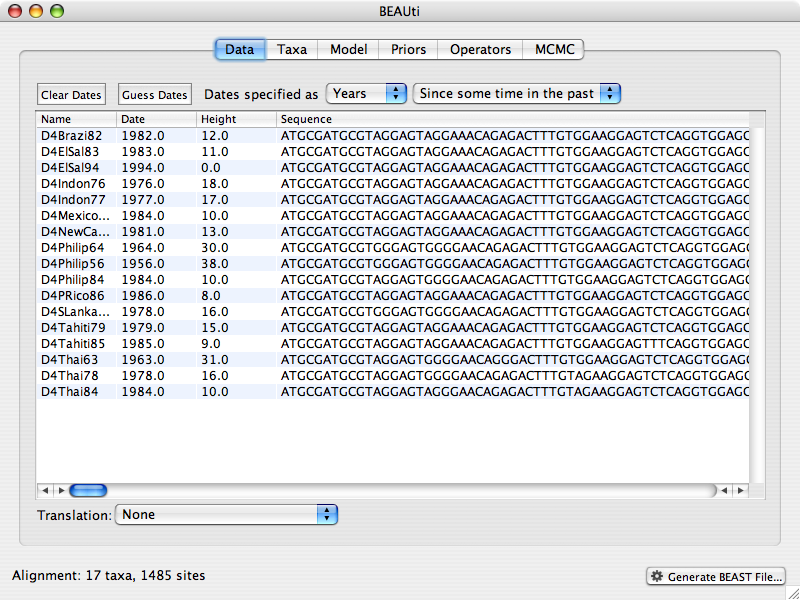
\includegraphics{Figure1_Data.png}}
\end{center}
\caption{The data tab in BEAUTi}
\label{fig:figure1}
\end{figure}

\section{Setting the dates of the taxa}

If the NEXUS file contains a calibrations block then the dates will automatically be loaded. Otherwise, by default 
all the taxa are assumed to have a date of zero (i.e. the sequences are assumed to be sampled at the same time). 
In this case, the dengue-4 virus have been sampled at various dates going back to the 1950s. The actual year of 
sampling is given in the name of each taxon and we could simply edit the value in the Date column of the table to
reflect these. However the following subsections describe two simpler methods for specifying the sequence dates.

\subsection{NEXUS Calibrations block}

One method for defining the tip calibrations in a serially sampled data set is to provide a calibrations block in
the NEXUS file to be imported. The following calibrations block is used in the  \texttt{Dengue4.env.nex} file:

\begin{verbatim}
  BEGIN CALIBRATION;
    OPTIONS SCALE = years;

    TIPCALIBRATION
      94 = 1994:D4ElSal94,
      86 = 1986:D4PRico86,
      85 = 1985:D4Tahiti85,
      84 = 1984:D4Mexico84 D4Philip84 D4Thai84,
      82 = 1982:D4Brazi82,
      83 = 1983:D4ElSal83,
      81 = 1981:D4NewCal81,
      79 = 1979:D4Tahiti79,
      78 = 1978:D4SLanka78 D4Thai78,
      77 = 1977:D4Indon77,
      76 = 1976:D4Indon76,
      64 = 1964:D4Philip64,
      63 = 1963:D4Thai63,
      56 = 1956:D4Philip56
      ;
  END;
\end{verbatim}

 The format within the \texttt{TIPCALIBRATION} command is a comma-delimited list of calibrations followed by a
 semicolon. Each calibration is of the form:

\begin{verbatim}
  calibration-name = calibration-date:taxa-list
\end{verbatim}

The  {\it taxa-list} is a space-delimited list of the taxa to be calibrated with the given calibration date.

\subsection{Guessing the dates from the taxa names}

If the taxa names contain the calibration information, then another convenient way to specify the dates of the
sequences in BEAUTi is to use the ``Guess Dates'' button at the top of the Data tab. Clicking this will make a
dialog box appear (Figure~\ref{fig:figure2}).

\begin{figure}[htbp]
\begin{center}
\leavevmode
\scalebox{0.4}{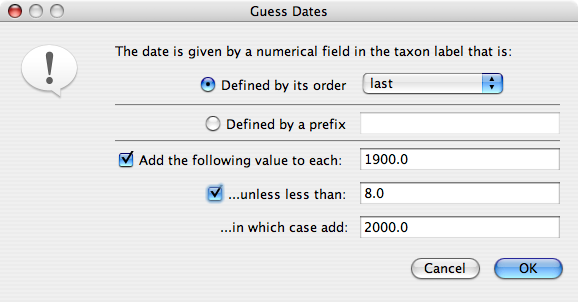
\includegraphics{Figure2_GuessDates.png}}
\end{center}
\caption{The Guess Dates dialog}
\label{fig:figure2}
\end{figure}

This operation attempts to guess what the dates are from information contained within the taxon names.
It works by trying to find a numerical field within each name. If the taxon names contain more than one
numerical field (such as the dengue-4 virus sequences, above) then you can specify how to find the one that
corresponds to the date of sampling. You can either specify the order that the date field comes (e.g.,
first, last or various positions in between) or specify a prefix (some characters that come immediately
before the date field in each name). For the dengue-4 sequences you select last from the drop-down menu
for the order. If you left it at first then all taxa would be given a date of "4" taken from the second
character of each name.

In this dialog box, you can also get BEAUti to add a fixed value to each guessed date. In this case the
value ``1900'' has been added to turn the dates from 2 digit years to 4 digit. Any dates in the taxon names
given as ``00'' would thus become ``1900''. If these dates were actually referring to the year 2000 then
selecting the next option would convert them correctly, adding 2000 to any date less than 08.
When you press OK the dates will appear in the appropriate column of the main window. You can then check
these and edit them manually as required. At the top of the window you can set the units that the dates
are given in (years, months, days) and whether they are specified relative to a point in the past (as
would be the case for years such as 1984) or backwards in time from the present (as in the case of
radiocarbon ages).

\subsection{Translating the data in amino acid sequences}

At the bottom of the main window is the option to translate the data into amino acid sequences. This will
be done using the genetic code specified in the associated drop down menu. If the loaded sequence are not
nucleotides then this option will be disabled.

\section{Setting the evolutionary model}

The next thing to do is to click on the Model tab at the top of the main window. This will reveal the
evolutionary model settings for BEAST. Exactly which options appear depend on whether the data are
nucleotides or amino acids (or nucleotides translated into amino acids). Figure~\ref{fig:figure3}
shows the settings that will appear after loading the dengue-4 data.

\begin{figure}[htbp]
\begin{center}
\leavevmode
\scalebox{0.4}{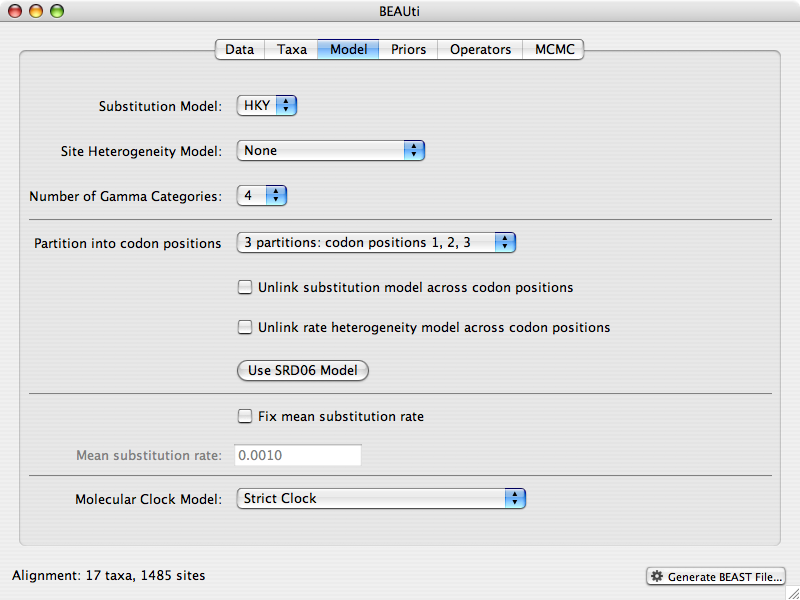
\includegraphics{Figure3_Model.png}}
\end{center}
\caption{The evolutionary model settings in BEAUTi}
\label{fig:figure3}
\end{figure}

This chapter assumes that you are familiar with the evolutionary models available, however there are
a couple of points to note about selecting a model in BEAUTi:

\begin{itemize}
\item Selecting the {\it Partition into codon positions} option assumes that the data are aligned
as codons. This option will then estimate a separate rate of substitution for each codon position,
or for 1+2 versus 3, depending on the setting.
\item Selecting the {\it Unlink substitution model across codon positions} will specify that BEAST
should estimate a separate transition-transversion ratio or general time reversible rate matrix for
each codon position.
\item Selecting the {\it Unlink rate heterogeneity model across codon positions} will specify that
BEAST should estimate set of rate heterogeneity parameters (gamma shape parameter and/or proportion
of invariant sites) for each codon position.
\item If there are no dates for the sequences (they are contemporaneous) then you can specify a
fixed {\it mean substitution rate} obtained from another source. Setting this to 1.0 will result
in the ages of the nodes of the tree being estimated in units of substitutions per site (i.e. the
normal units of branch lengths in popular packages such as MRBAYES).
\end{itemize}

\section{Setting up the operators}

Each parameter in the model has one or more``operators" (these are variously called moves and
proposals by other MCMC software packages such as MRBAYES and LAMARC). The operators specify how
the parameters change as the MCMC runs. The operators tab in BEAUti has a table that lists the parameters,
their operators and the tuning settings for these operators. In the first column are the parameter names.
These will be called things like \texttt{hky.kappa} which means the HKY model's kappa parameter (the
transition-transversion bias). The next column has the type of operators that are acting on each
parameter. For example, the scale operator scales the parameter up or down by a proportion, the
random walk operator adds or subtracts an amount to the parameter and the uniform operator simply
picks a new value uniformly within a range. Some parameters relate to the tree or to the divergence
times of the nodes of the tree and these have special operators.

The next column, labelled {\it Tuning}, gives a tuning setting to the operator. Some operators
don't have any tuning settings so have {\it n/a} under this column. The tuning parameter will
determine how large a move each operator will make which will affect how often that change is
accepted by the MCMC which will affect the efficency of the analysis. For most operators (like
random walk and subtree slide operators) a larger tuning parameter means larger moves. However
for the scale operator a tuning parameter value closer to 0.0 means bigger moves. At the top of
the window is an option called {\it Auto Optimize} which, when selected, will automatically adjust
the tuning setting as the MCMC runs to try to achieve maximum efficiency. At the end of the run
a table of the operators, their performance and the final values of these tuning settings will be
written to standard ouput. These can then be used to set the starting tuning settings in order to
minimize the amount of time taken to reach optimum performance in subsequent runs.

The next column, labelled {\it Weight}, specifies how often each operator is applied relative
to the others. Some parameters tend to be sampled very efficiently - an example is the kappa
parameter - these parameters can have their operators down-weighted so that they are not changed
as often (this may mean upweighting other operators since the weights must be integers).

\section{Setting the MCMC options}

The {\it MCMC} tab in BEAUTi provides settings to control the MCMC chain (Figure~\ref{fig:figure4}). Firstly we have the
{\it Length of chain}. This is the number of steps the MCMC will make in the chain before
finishing. How long this should be depends on the size of the dataset, the complexity of the
model and the precision of the answer required. The default value of 10,000,000 is entirely
arbitrary and should be adjusted according to the size of your dataset. In order to examine
whether a particular chain length is adequate, the resulting log file can be analysed using
TRACER. The aim is to set the chain length so as to achieve an adequate effective sample
size (ESS).

The next couple of options specify how often the current parameter values should be displayed
on the screen and recorded in the log file. The screen output is simply for monitoring the
programs progress so can be set to any value (although if set too small, the sheer quantity
of information being displayed on the screen will slow the program down). For the log
file, the value should be set relative to the total length of the chain. Sampling too often
will result in very large files with little extra benefit in terms of the precision of the
estimates. Sample too infrequently and the log file will not contain much information about
the distributions of the parameters. You probably want to aim to store no more than 10,000
samples so this should be set to the chain length / 10,000. For this dataset let's initially
setting the chain length to 100,000 as this will run reasonably quickly on most modern
computers. The final two options give the file names of the log files for the parameters and the trees.
These will be set to a default based on the name of the imported NEXUS file but feel free
to change these.

\begin{figure}[htbp]
\begin{center}
\leavevmode
\scalebox{0.4}{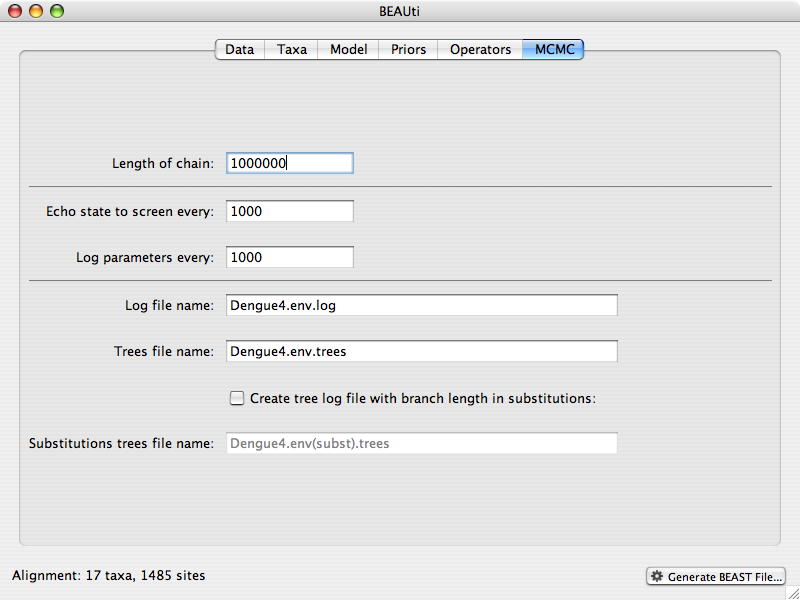
\includegraphics{Figure4_MCMC.png}}
\end{center}
\caption{The MCMC settings in BEAUTi}
\label{fig:figure4}
\end{figure}

\section{Running BEAST}

At this point we are ready to generate a BEAST XML file and to use this to run the Bayesian
evolutionary analysis. To do this, either select the {\it Generate BEAST File...} option
from the File menu or click the similarly labelled button at the bottom of the window.
Choose a name for the file (for example, \texttt{Dengue4.env.xml}) and save the file. For
convenience, leave the BEAUti window open so that you can change the values and re-generate
the BEAST file as required later in this tutorial.

\section{Analysing the BEAST output}

To analyse the results of running BEAST we are going to use the program TRACER.
The exact instructions for running Tracer differs depending
on which computer you are using. Please see the README text file that was distributed with the
version you downloaded. Once running, Tracer will look similar irrespective of which computer system
it is running on.

Select the Open option from the File menu. If you have it available, select the log file
that you created in the previous section. The file will load and you will be
presented with a window similar to the one below (Figure~\ref{fig:figure5}). Remember that MCMC is a stochastic
algorithm so the actual numbers will not be exactly the same.

\begin{figure}[htbp]
\begin{center}
\leavevmode
\scalebox{0.3}{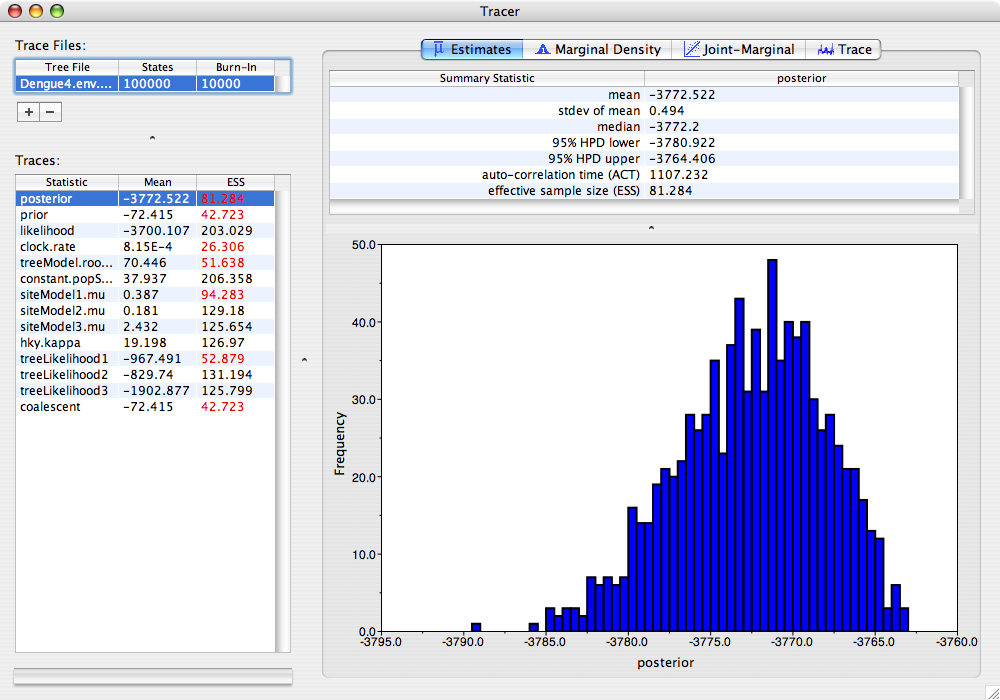
\includegraphics{Figure5_Tracer1.png}}
\end{center}
\caption{The main Tracer window with a BEAST log file loaded.}
\label{fig:figure5}
\end{figure}

On the left hand side is the name of the log file loaded and the traces that it contains.
There are traces for the posterior (this is the log of the product of the tree likelihood and
the prior probabilities), and the continuous parameters. Selecting a trace on the left
brings up analyses for this trace on the right hand side depending on tab that is
selected. When first opened (Figure~\ref{fig:figure5}), the `posterior' trace is selected and various statistics
of this trace is shown under the Estimates tab.

Note that the effective sample sizes (ESSs) for all the traces are small (ESSs less than
100 are highlighted in red by Tracer). This is not good. A low ESS means that the trace
contained a lot of correlated samples and thus may not represent the posterior distribution
well. In the bottom right of the window is a frequency plot of the samples which as
expected given the low ESSs is extremely rough (Figure~\ref{fig:figure5}).

In the top right of the window is a table of calculated statistics for the selected trace.
The statistics and their meaning are described in the table below.

\begin{itemize}
\item {\it Mean} -
The mean value of the samples (excluding the burn-in).
\item {\it Stdev} -
The standard error of the mean. This takes into account the effective sample size so a
small ESS will give a large standard error.
\item {\it Median} -
The median value of the samples (excluding the burn-in).
\item {\it 95\% HPD Lower} -
The lower bound of the highest posterior density (HPD) interval. The HPD is the shortest interval
that contains 95\% of the sampled values.
\item {\it 95\% HPD Upper} -
The upper bound of the highest posterior density (HPD) interval. The HPD is the shortest interval
that contains 95\% of the sampled values.
\item {\it Auto-Correlation Time (ACT)} -
The average number of states in the MCMC chain that two samples have to be separated by for them
to be uncorrelated (i.e. independent samples from the posterior). The ACT is estimated from the
samples in the trace (excluding the burn-in).
\item {\it Effective Sample Size (ESS)} -
The ESS is the number of independent samples that the trace is equivalent to. This is
calculated as the chain length (excluding the burn-in) divided by the ACT.
\end{itemize}

If we select the tab on the right-hand-side labelled `Trace' we can view the raw trace,
that is, the sampled values against the  step in the MCMC chain (Figure~\ref{fig:figure6}).

\begin{figure}[htbp]
\begin{center}
\leavevmode
\scalebox{0.3}{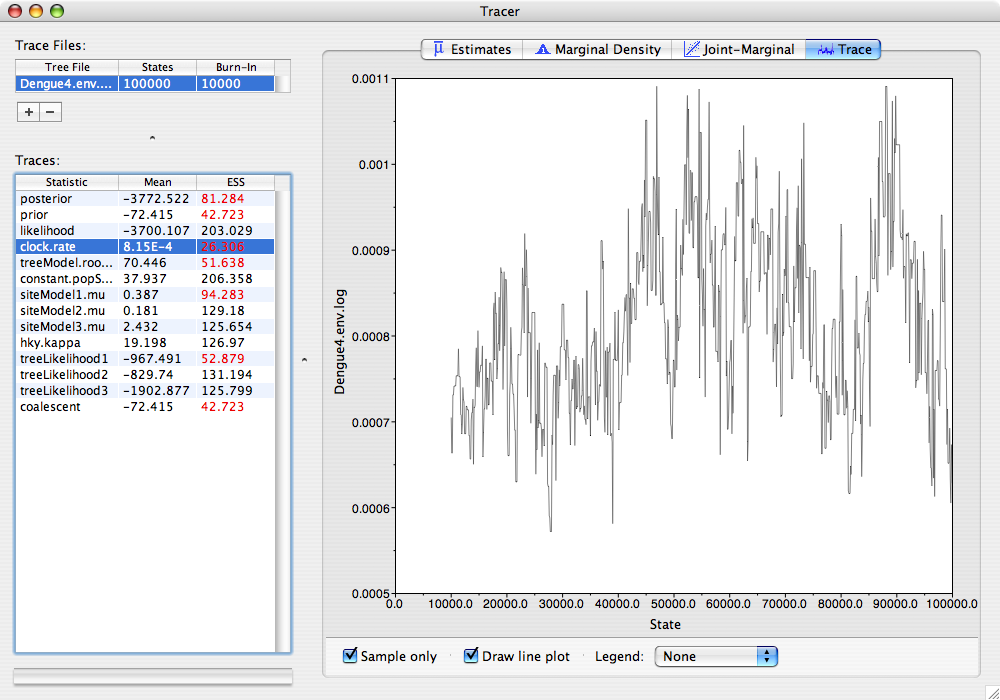
\includegraphics{Figure6_Tracer2.png}}
\end{center}
\caption{The trace of posterior against chain length in TRACER for a run of 100,000 steps.}
\label{fig:figure6}
\end{figure}

Here you can see how the samples are correlated. There are 1000 samples in the trace
(we ran the MCMC for 100,000 steps sampling every 100) but it is clear that adjacent
samples often tend to have similar values. The ESS for the likelihood is about 80 so we
are only getting 1 independent sample to every 12 actual samples. It also seems
that the default burn-in of 10\% of the chain length is inadequate. Not excluding enough
of the start of the chain as burn-in will bias the results and render estimates of ESS
unreliable.

The simple response to this situation is that we need to run the chain for longer. Given the lowest
ESS (for the \texttt{clock.rate}) is 26, it would suggest that we have to run it at least 4
times longer to get ESSs that are $>$100. However it would be better to aim higher so lets
go for a chain length of 1,000,000. Go back to Section \ref{section:2.7}
and create a new BEAST XML file with a longer chain length. Now run BEAST and load the new
log file into Tracer (you can leave the old one loaded for comparison). Click on the Trace
tab and look at the raw trace plot (Figure~\ref{fig:figure7}).

\begin{figure}[htbp]
\begin{center}
\leavevmode
\scalebox{0.3}{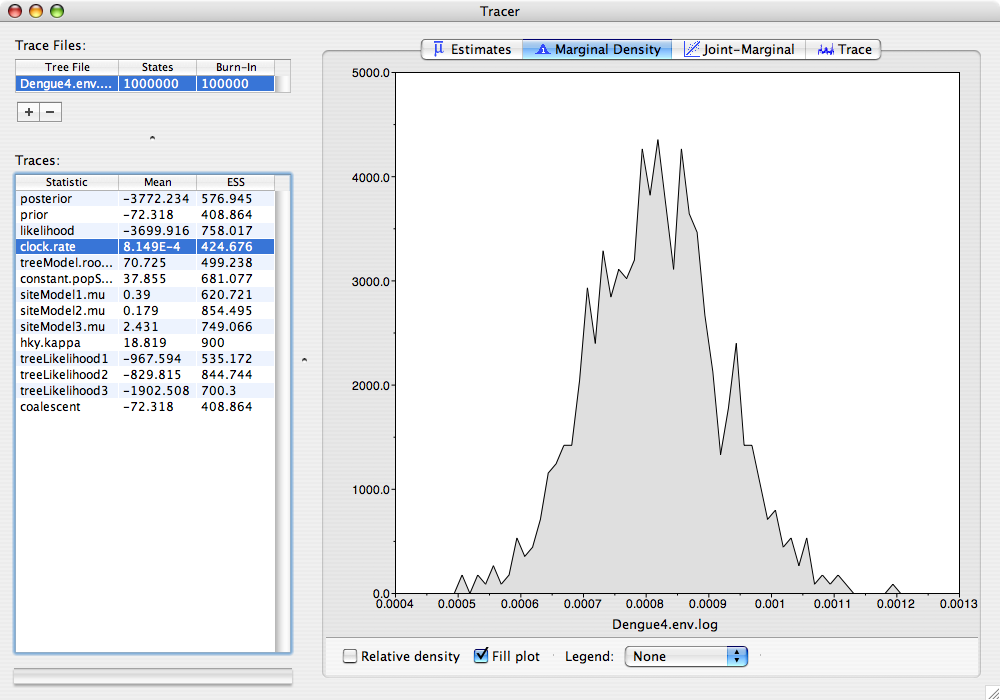
\includegraphics{Figure7_Tracer3.png}}
\end{center}
\caption{The trace of posterior against chain length in Tracer for a run of 1,000,000 steps.}
\label{fig:figure7}
\end{figure}

Again we have chosen options that produce 1000 samples and with an ESS
of about 500 there is still auto-correlation between the samples but 500 effectively independent
samples will now provide a good estimate of the posterior distribution. There are no obvious trends
in the plot suggesting that the MCMC was
still converging and there are no large-scale fluctuations in the trace suggesting poor
mixing.
As we are happy with the behaviour of log-likelihood we can now move on to one of the
parameters of interest: substitution rate. Select \texttt{clock.rate} in the left-hand table. This
is the mutation rate of the first codon position. Now choose the density plot by selecting
the tab labeled Density. This shows a plot of the posterior probability density of this
parameter. You should see a plot similar to Figure~\ref{fig:figure8}.

\begin{figure}[htbp]
\begin{center}
\leavevmode
\scalebox{0.3}{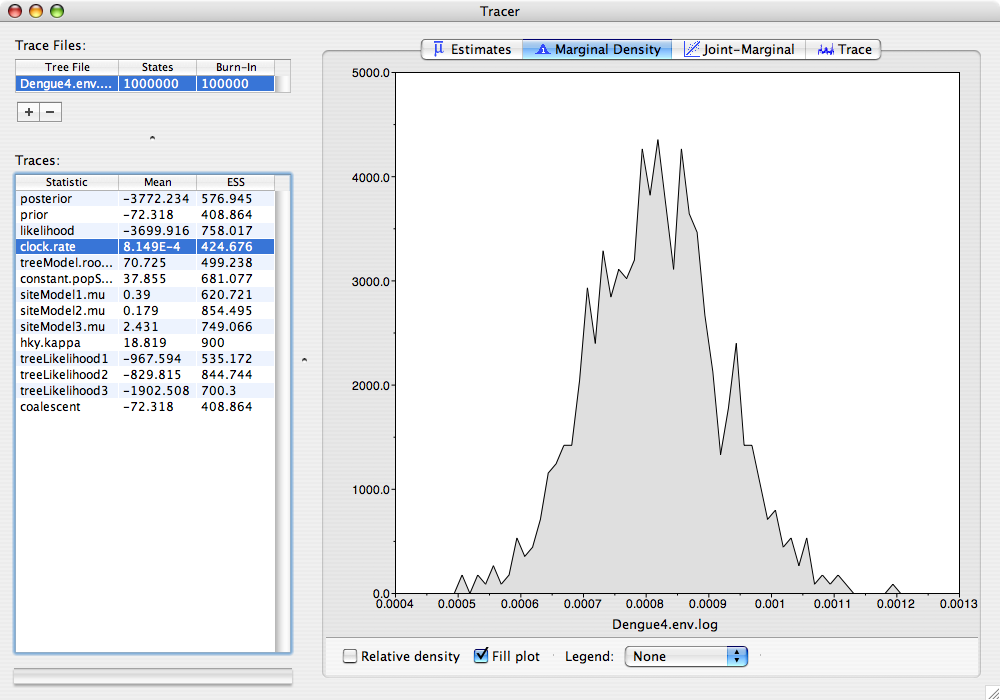
\includegraphics{Figure8_Tracer4.png}}
\end{center}
\caption{The posterior density plot for the subtitution rate.}
\label{fig:figure8}
\end{figure}

As you can see the posterior probability density is roughly bell-shaped.
There is some sampling noise which would be reduced if we ran the chain for longer but
we already have a good estimate of the mean and HPD interval. You can overlay
the density plots of multiple traces in order to compare them (it is up to the user to determine
whether they are comparable on the the same axis or not). Select the relative substitution rates for all three
codon positions in the table to the left (labelled \texttt{siteModel1.mu}, \texttt{siteModel2.mu} and \texttt{siteModel3.mu}. You will now see
the posterior probability densities for the relative substitution rate at all three codon positions
over-layed (Figure~\ref{fig:figure9}).

\begin{figure}[htbp]
\begin{center}
\leavevmode
\scalebox{0.3}{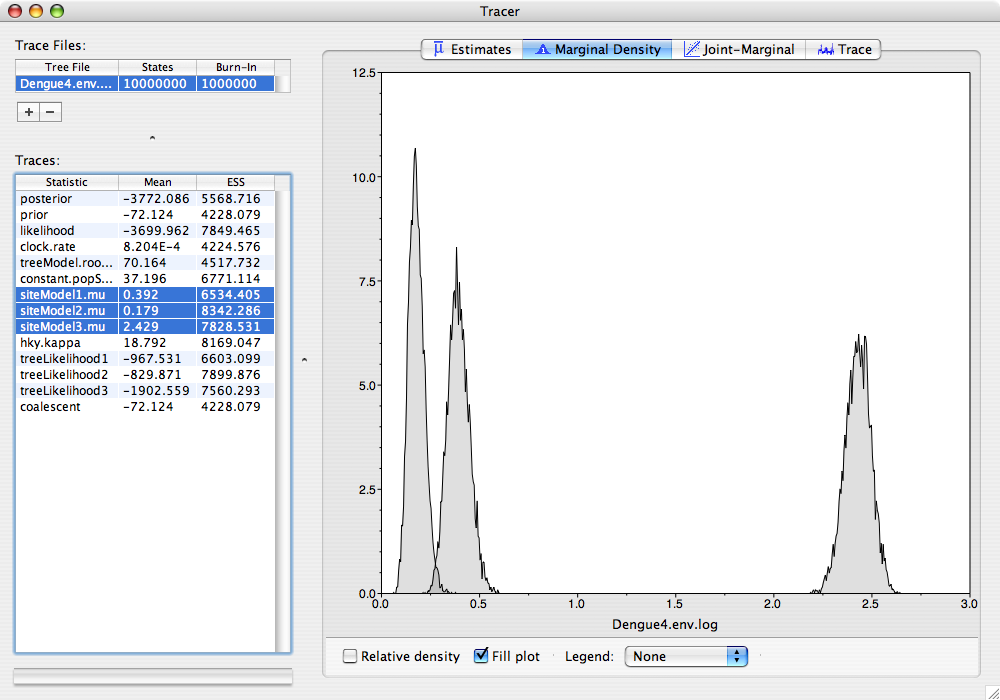
\includegraphics{Figure9_Tracer5.png}}
\end{center}
\caption{The posterior density plots for the relative rate of evolution at each
codon position.}
\label{fig:figure9}
\end{figure}

\section{Summarizing the trees}

We have seen how we can diagnose our MCMC run using Tracer and produce estimates of the
marginal posterior distributions of parameters of our model. However, BEAST also samples
trees (either phylogenies or geneologies) at the same time as the other parameters
of the model. These are written to a separate file called the `trees' file. This
file is a standard NEXUS format file. As such it can easily be loaded into other
software in order to examine the trees it contains. One possibility is to load the
trees into a program such as PAUP* and construct a consensus tree in a similar manner
to summarizing a set of bootstrap trees. In this case, the support values reported
for the resolved nodes in the consensus tree will be the posterior probability of
those clades.

In this tutorial, however, we are going to use a tool that is provided as part
of the BEAST package to summarize the information contained within our sampled
trees. The tool is called `TreeAnnotator' and once running, you will be presented with a
window like the one in Figure~\ref{fig:figure10}.

\begin{figure}[htbp]
\begin{center}
\leavevmode
\scalebox{0.4}{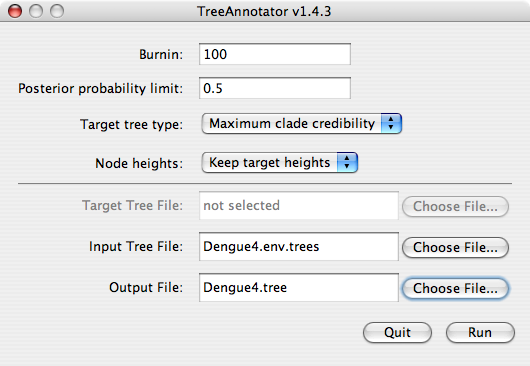
\includegraphics{Figure10_TreeAnnotator.png}}
\end{center}
\caption{The user-interface for the TreeAnnotator tool.}
\label{fig:figure10}
\end{figure}

TreeAnnotator takes a single `target' tree and annotates it with the summarized
information from the entire sample of trees. The summarized information includes
the average node ages (along with the HPD intervals), the posterior
support and the average rate of evolution on each branch (for models where this
can vary). The program calculates these values for each node or clade observed in
the specified 'target' tree.

\begin{itemize}
\item {\it Burnin} -
This is the number of trees in the input file that should be excluded from the summarization.
This value is given as the number of trees rather than the number of steps in the MCMC chain.
Thus for the example above, with a chain of 1,000,000 steps, sampling every 1000 steps, there
are 1000 trees in the file. To obtain a 10\% burnin, set this value to 100.
\item {\it Posterior probability limit} -
This is the minimum posterior probability for a node in order for TreeAnnotator to store
the annoted information. The default is 0.5 so only nodes with this posterior probability
or greater will have information summarized (the equivalent to the nodes in a majority-rule
consensus tree). Set this value to 0.0 to summarize all nodes in the target tree.
\item {\it Target tree type} -
This has two options "Maximum clade credibility" or "User target tree". For the latter option,
a NEXUS tree file can be specified as the Target Tree File, below. For the former option,
TreeAnnotator will examine every tree in the Input Tree File and select the tree that has
the highest sum of the posterior probabilities of all its nodes.
\item {\it Node heights} -
This option specifies what node heights (times) should be used for the output tree. If the ``Keep
target heights'' is selected, then the node heights will be the same as the target tree. The other
two options give node heights as an average (Mean or Median) over the sample of trees.
\item {\it Target Tree File} -
If the "User target tree" option is selected then you can use "Choose File..." to select a
NEXUS file containing the target tree.
\item {\it Input Tree File} -
Use the "Choose File..." button to select an input trees file. This will be the trees file
produced by BEAST.
\item {\it Output File} -
Select a name for the output tree file.
\end{itemize}

Once you have selected all the options, above, press the "Run" button. TreeAnnotator will analyse
the input tree file and write the summary tree to the file you specified. This tree is in
standard NEXUS tree file format so may be loaded into any tree drawing package that supports this.
However, it also contains additional information that can only be displayed using the FigTree
program.

\section{Viewing the annotated tree}

Run FigTree now and select the {\it Open...} command from the {\it File} menu. Select the tree file
you created using TreeAnnotator in the previous section. The tree will be displayed in the FigTree
window. On the left hand side of the window are the options and setting which control how the
tree is displayed. In this case we want to display the posterior probabilities of each of the clades
present in the tree and estimates of the age of each node (see Figure~\ref{fig:figure11}). In order
to do this you need to change some of the settings.

\begin{figure}[htbp]
\begin{center}
\leavevmode
\scalebox{0.3}{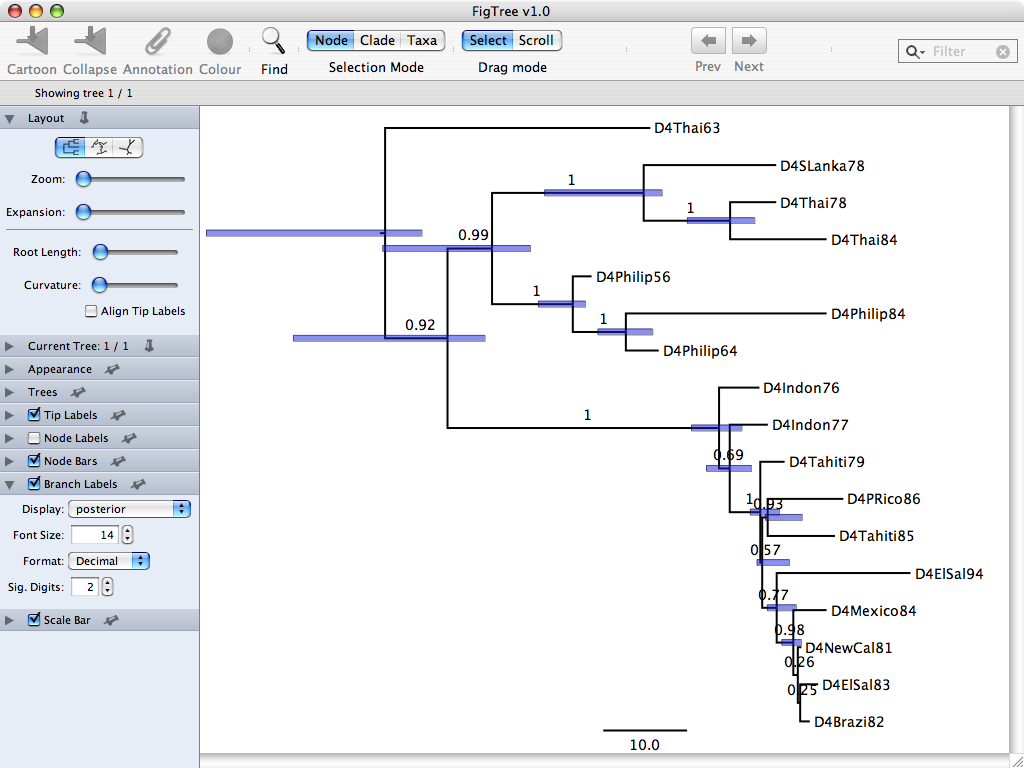
\includegraphics{Figure11_FigTree.png}}
\end{center}
\caption{The annotated tree displayed in FigTree.}
\label{fig:figure11}
\end{figure}

First open the {\it Branch Labels} section of
the control panel on the left. Now select {\it posterior} from the {\it Display} popup menu. The
posterior probabilities won't actually be displayed until you tick the check-box next to the
{\it Branch Labels} title.

We now want to display bars on the tree to represent the estimated uncertainty in the date for
each node. TreeAnnotator will have placed this information in the tree file in the shape of the
95\% highest posterior density (HPD) intervals (see the description of HPDs, above). Open the
{\it Node Bars} section of the control panel and you will notice that it is already
set to display the 95\% HPDs of the node heights so all you need to do is to select the check-box in
order to turn the node bars on.

Finally, open the {\it Appearance} panel and alter the {\it Line Weight} to draw the tree with thicker
lines. None of the options actually alter the tree's topology or branch lengths in anyway so feel free
to explore the options and settings. You can also save the tree and this will save all your settings
so that when you load it into FigTree again it will be displayed exactly as you selected.

\section{Conclusion and Resources}

This chapter only scratches the surface of the analyses that are possible to undertake using
BEAST. It has hopefully provided a relatively gentle introduction to the fundimental steps that will
be common to all BEAST analyses and provide a basis for more challenging investigations. BEAST is an
ongoing development project with new models and techniques being added on a regular basis. The BEAST website
provides details of the mailing list that is used to announce new features and to discuss the use
of the package. The website also contains a list of tutorials and recipes
 to answer particular evolutionary questions using BEAST as well as a description of the XML
input format, common questions and error messages.

 \begin{itemize}
 \item The BEAST website:
 http://beast.bio.ed.ac.uk/
 \item Tutorials:
 http://beast.bio.ed.ac.uk/Tutorials/
 \item Frequently asked questions:
 http://beast.bio.ed.ac.uk/FAQ/
 \end{itemize}

\begin{thebibliography}{77}
\bibitem{HR2001}Huelsenbeck JP, Ronquist F: MRBAYES: Bayesian inference
of phylogenetic trees. \emph{Bioinformatics} 2001, \textbf{17}:754-755.

\bibitem{DNRS2002}Drummond AJ, Nicholls GK, Rodrigo AG, Solomon W:
Estimating mutation parameters, population history and genealogy simultaneously
from temporally spaced sequence data. \emph{Genetics} 2002, \textbf{\noun{161}}(3):1307-1320.

\bibitem{WWB2003}Wilson IJ, Weale ME, Balding DJ: Inferences from
DNA data: population histories, evolutionary processes and forensic
match probabilities. \emph{J Royal Stat Soc A-Statistics in Society}
2003, \textbf{166}:155-188.

\bibitem{Beaumont1999}Beaumont MA: Detecting population expansion
and decline using microsatellites. \emph{Genetics} 1999, \textbf{153}(4):2013-2029.

\bibitem{RY2003}Rannala B, Yang ZH: Bayes estimation of species divergence
times and ancestral population sizes using DNA sequences from multiple
loci. \emph{Genetics} 2003, \textbf{164}(4):1645-1656.

\bibitem{PDNRR2003}Pybus OG, Drummond AJ, Nakano T, Robertson BH,
Rambaut A: The epidemiology and iatrogenic transmission of hepatitis
C virus in Egypt: a Bayesian coalescent approach. \emph{Mol Biol Evol}
2003, \textbf{20}(3):381-387.

\bibitem{Kuhner2006}Kuhner, MK: LAMARC 2.0: Maximum likelihood and
Bayesian estimation of population parameters. \emph{Bioinformatics}
2006 \textbf{22}(6):768-770.

\bibitem{RS2005}Redelings BD, Suchard MA: Joint Bayesian Estimation
of Alignment and Phylogeny. \emph{Syst Biol} 2005, \textbf{54}(3):401-418.

\bibitem{LMDJH2005}Lunter G, Miklos I, Drummond A, Jensen JL, Hein
J: Bayesian coestimation of phylogeny and sequence alignment. \emph{BMC
Bioinformatics} 2005, \textbf{6}(1):83.

\bibitem{Hastings1970}Hastings WK: Monte Carlo sampling methods using
Markov chains and their applications. \emph{Biometrika} 1970, \textbf{57}:97-109.

\bibitem{MRRTT1953}Metropolis N, Rosenbluth A, Rosenbluth M, Teller
A, Teller E: Equations of state calculations by fast computing machines.
\emph{J Chem Phys} 1953, \textbf{21}:1087-1091.

\bibitem{ZP1965}Zuckerkandl E, Pauling L: Evolutionary divergence
and convergence in proteins. In: \emph{Evolving genes and proteins}.
Edited by Bryson V, Vogel HJ. Academic Press: New York; 1965: 97-166.

\bibitem{AY2003}Aris-Brosou S, Yang Z: Bayesian models of episodic
evolution support a late Precambrian explosive diversification of
the Metazoa. \emph{Mol Biol Evol} 2003, \textbf{20}(12):1947-1954.

\bibitem{KTB2001}Kishino H, Thorne JL, Bruno WJ: Performance of a
divergence time estimation method under a probabilistic model of rate
evolution. Molecular Biology \& Evolution 2001, 18:352-361.

\bibitem{Sanderson2002}Sanderson MJ: Estimating absolute rates of
molecular evolution and divergence times: A penalized likelihood approach.
\emph{Mol Biol Evol} 2002, \textbf{19}:101-109.

\bibitem{TK2002}Thorne JL, Kishino H: Divergence time and evolutionary
rate estimation with multilocus data. \emph{Syst Biol} 2002, \textbf{51}(5):689-702.

\bibitem{TKP1998}Thorne JL, Kishino H, Painter IS: Estimating the
rate of evolution of the rate of molecular evolution. \emph{Mol Biol
Evol} 1998, \textbf{15}:1647-1657.

\bibitem{YY2000}Yoder AD, Yang ZH: Estimation of primate speciation
dates using local molecular clocks. \emph{Mol Biol Evol} 2000, \textbf{17}:1081-1090.

\bibitem{SR2006}Suchard MA, Redelings BD: BAli-Phy: simultaneous
Bayesian inference of alignment and phylogeny. \emph{Bioinformatics}
2006 \textbf{22}(16):2047-2048.

\bibitem{RD2003}Rambaut A, Drummond AJ: Tracer {[}computer program]
Available from http://evolve.zoo.ox.ac.uk/software/ 2003

\bibitem{Shapiroetal2004}Shapiro B, Drummond AJ, Rambaut A, Wilson
MC, Matheus PE, Sher AV, Pybus OG, Gilbert MT, Barnes I, Binladen
J et al: Rise and fall of the Beringian steppe bison. \emph{Science}
2004, \textbf{306}(5701):1561-1565.

\bibitem{ROMM1990}Rodriguez F, Oliver JL, Marin A, Medina JR: The
general stochastic model of nucleotide substitution. \emph{J Theor
Biol} 1990, \textbf{142}(4):485-501.

\bibitem{HKY1985}Hasegawa M, Kishino H, Yano T: Dating of the human-ape
splitting by a molecular clock of mitochondrial DNA. \emph{J Mol Evol}
1985, \textbf{22}(2):160-174.

\bibitem{GY1994}Goldman N, Yang Z: A codon-based model of nucleotide
substitution for protein-coding DNA sequences. \emph{Mol Biol Evol}
1994, \textbf{11}(5):725-736.

\bibitem{Y1994}Yang Z: Maximum likelihood phylogenetic estimation
from DNA sequences with variable rates over sites: approximate methods.
\emph{J Mol Evol} 1994, \textbf{39}(3):306-314.

\bibitem{DPRFR2003}Drummond AJ, Pybus OG, Rambaut A, Forsberg R,
Rodrigo AG: Measurably evolving populations. \emph{Trends Ecol Evol}
2003, \textbf{18}(9):481-488.

\bibitem{GT1994}Griffiths RC, Tavare S: Sampling theory for neutral
alleles in a varying environment. \emph{Philos Trans R Soc Lond B
Biol Sci} 1994, \textbf{344}(1310):403-410.

\bibitem{Kingman1982}Kingman JFC: The coalescent. \emph{Stochastic
Processes and Their Applications} 1982, \textbf{13}:235-248.

\bibitem{DRSP2005}Drummond AJ, Rambaut A, Shapiro B, Pybus OG: Bayesian
coalescent inference of past population dynamics from molecular sequences.
\emph{Mol Biol Evol} 2005, \textbf{22}(5):1185-1192.

\bibitem{Aldous2001}Aldous DJ: Stochastic models and descriptive
statistics for phylogenetic trees, from Yule to today. \emph{Statistical
Science} 2001, \textbf{16}(1):23-34.

\bibitem{DHPR2006}Drummond AJ, Ho SYW, Phillips MJ, Rambaut A: Relaxed
phylogenetics and dating with confidence. \emph{PLoS Biology} 2006,
\textbf{4}(5)

\bibitem{TKF1991}Thorner JL, Kishino H, Felsenstein J: An evolutionary
model for maximum likelihood alignment of DNA sequences. \emph{J Mol
Evol} 1991, \textbf{33}(2): 114-124.

\bibitem{Lemeyetal2004}Lemey P, Pybus OG, Rambaut A, Drummond AJ,
Robertson DL, Roques P, Worobey M, Vandamme AM: The molecular population
genetics of HIV-1 group O. \emph{Genetics} 2004, \textbf{167}(3):1059-1068.

\bibitem{LGT1997}Lanciotti RS, Gubler DJ, Trent DW: Molecular evolution and
phylogeny of dengue-4 viruses.  \emph{Journal of General Virology} 1997,
\textbf{78}:2279-2284.

\bibitem{R2000}Rambaut A: Estimating the rate of molecular evolution: incorporating
non-contemporaneous sequences into maximum likelihood phylogenies.
\emph{Bioinformatics} 2000, \textbf{16}(4):395-399.

\end{thebibliography}

\end{document}
